
\chapter{基于监督学习的智能协议与参数联合选择方法}
\label{chapter5: ai_selector}

现代无线网络，尤其是物联网场景，业务需求呈现出显著的多样性与动态性。不同业务在接入密度、数据包长度及时延敏感度等方面差异明显，使得单一随机接入协议难以在复杂多变的网络条件下始终保持最优性能。传统基于固定协议与静态参数配置的设计，难以同时兼顾吞吐量、时延、公平性、信令开销多维性能指标，存在明显局限。
不同随机接入协议在吞吐性能、时延特性、信令开销方面表现各异。表~\ref{tab:protocol_comparison} 对 Slotted ALOHA(SA)、CBA、SAST典型协议进行了定性对比，可以看出，协议机制的增强虽可显著提升系统吞吐，但同时也可能带来更高的信令开销，进一步表明难以依靠单一协议适应所有场景。

\begin{table}[htbp]
\centering
\caption{不同随机接入协议的定性性能对比}
\label{tab:protocol_comparison}
\renewcommand{\arraystretch}{1.2}
\begin{tabular}{c|c|c|c}
\hline
\textbf{协议} & \textbf{吞吐性能} & \textbf{时延特性} & \textbf{信令开销} \\
\hline
SA & 低 & 低 & 中 \\
\hline
SAST & 中 & 中 & 低 \\
\hline
CBA & 高 & 中-高 & 高 \\
\hline

\end{tabular}
\end{table}


因此，依据场景特征动态选择接入协议并联合优化其关键参数，成为提升系统整体性能的有效途径。围绕这一需求，本章研究如何在多协议共存的统一框架下，根据业务流量状态智能决策最优协议及其参数配置。
针对此问题，本文提出一种面向复杂业务场景的、基于监督学习的协议与参数联合选择方法，旨在实现网络接入策略由静态配置向环境感知与数据驱动决策的转变，从而在吞吐量、时延与公平性等多维性能之间取得更优平衡。

\section{问题建模与统一接入框架设计}
本章在第二章第2.3节提出的通用上行网络模型基础上，构建了一种支持多协议并存与运行时动态切换的统一随机接入框架。在该框架下，节点可在运行过程中根据当前网络状态选择适宜的接入协议并配置相应参数。值得注意的是，节点的流量到达模式可能是均匀到达，也可能是突发到达，这取决于环境的变化和业务需求的动态特性。这种动态特性，使得以往单一传统的协议理论性能分析变得更加复杂和困难。


% 该统一框架的核心目标是将各类随机接入协议抽象为若干可调度、可配置的统计接入模式，并以网络的统计特征，尤其是业务流量的时序与分布属性，作为驱动信号，决策协议类型及其关键参数的自适应调整。通过将接入机制的设计从传统的协议逻辑层提升到统计建模与决策层，本框架为后续引入监督学习等数据驱动的方法提供了统一、可扩展的理论支撑与工程实现路径。

\subsection{问题建模}

为便于后续章节统一叙述，这里首先对问题进行简要建模。对于任意网络场景，我们用统一输入向量 $\mathbf{X}_{\mathrm{in}}$ 表征其关键配置与状态特征，包括业务流量特征、网络规模以及可选接入协议的候选范围及协议参数等。

在给定 $\mathbf{X}_{\mathrm{in}}$ 后，我们通过统一仿真器或监督学习代理模型评估该配置下的系统性能。记该评估过程为一个映射 $S(\cdot)$，其输出为多维性能指标向量 $\mathbf{y}=S\big(\mathbf{X}_{\mathrm{in}}\big)$。为便于跨场景与跨协议比较，引入归一化算子 $\mathrm{norm}(\cdot)$，得到归一化后的指标向量 $\tilde{\mathbf{y}}=\mathrm{norm}(\mathbf{y})$。在此基础上，用综合效用函数 $U(\cdot)$ 将 $\tilde{\mathbf{y}}$ 映射为单一的效用得分。

在上述定义下，我们希望从若干候选接入协议及其允许的参数配置中，选出使综合效用最大的那一组。该联合选择问题可形式化表述为：
\begin{equation}
\label{eq:chap5_overview}
\mathbf{x}_{\mathrm{proto}}^*
=\arg\max_{\mathbf{x}_{\mathrm{proto}}}
U\!\left(\mathrm{norm}\!\left(S\big(\mathbf{X}_{\mathrm{in}}\big)\right)\right),
\end{equation}
其中决策变量为统一参数向量 $\mathbf{x}_{\mathrm{proto}}$，其首个分量为协议类型标识符，其余分量为对应协议参数。记 $\mathbf{x}_{\mathrm{proto}} = [a, \mathbf{x}_p^{\top}]^{\top}$，其中 $a \in \mathcal{P}$ 表示从候选集合中选取的协议类型，$\mathbf{x}_p \in \mathcal{X}_p$ 为该协议的参数向量，$\mathcal{X}_a$ 为协议 $a$ 的合法参数空间。图~\ref{fig:chap5_framework} 给出了统一接入框架及协议选择流程的示意，后续内容将围绕式~\eqref{eq:chap5_overview} 分别展开统一输入构造、性能指标与效用定义以及数据驱动决策方法的设计。
\begin{figure}[t]
\centering
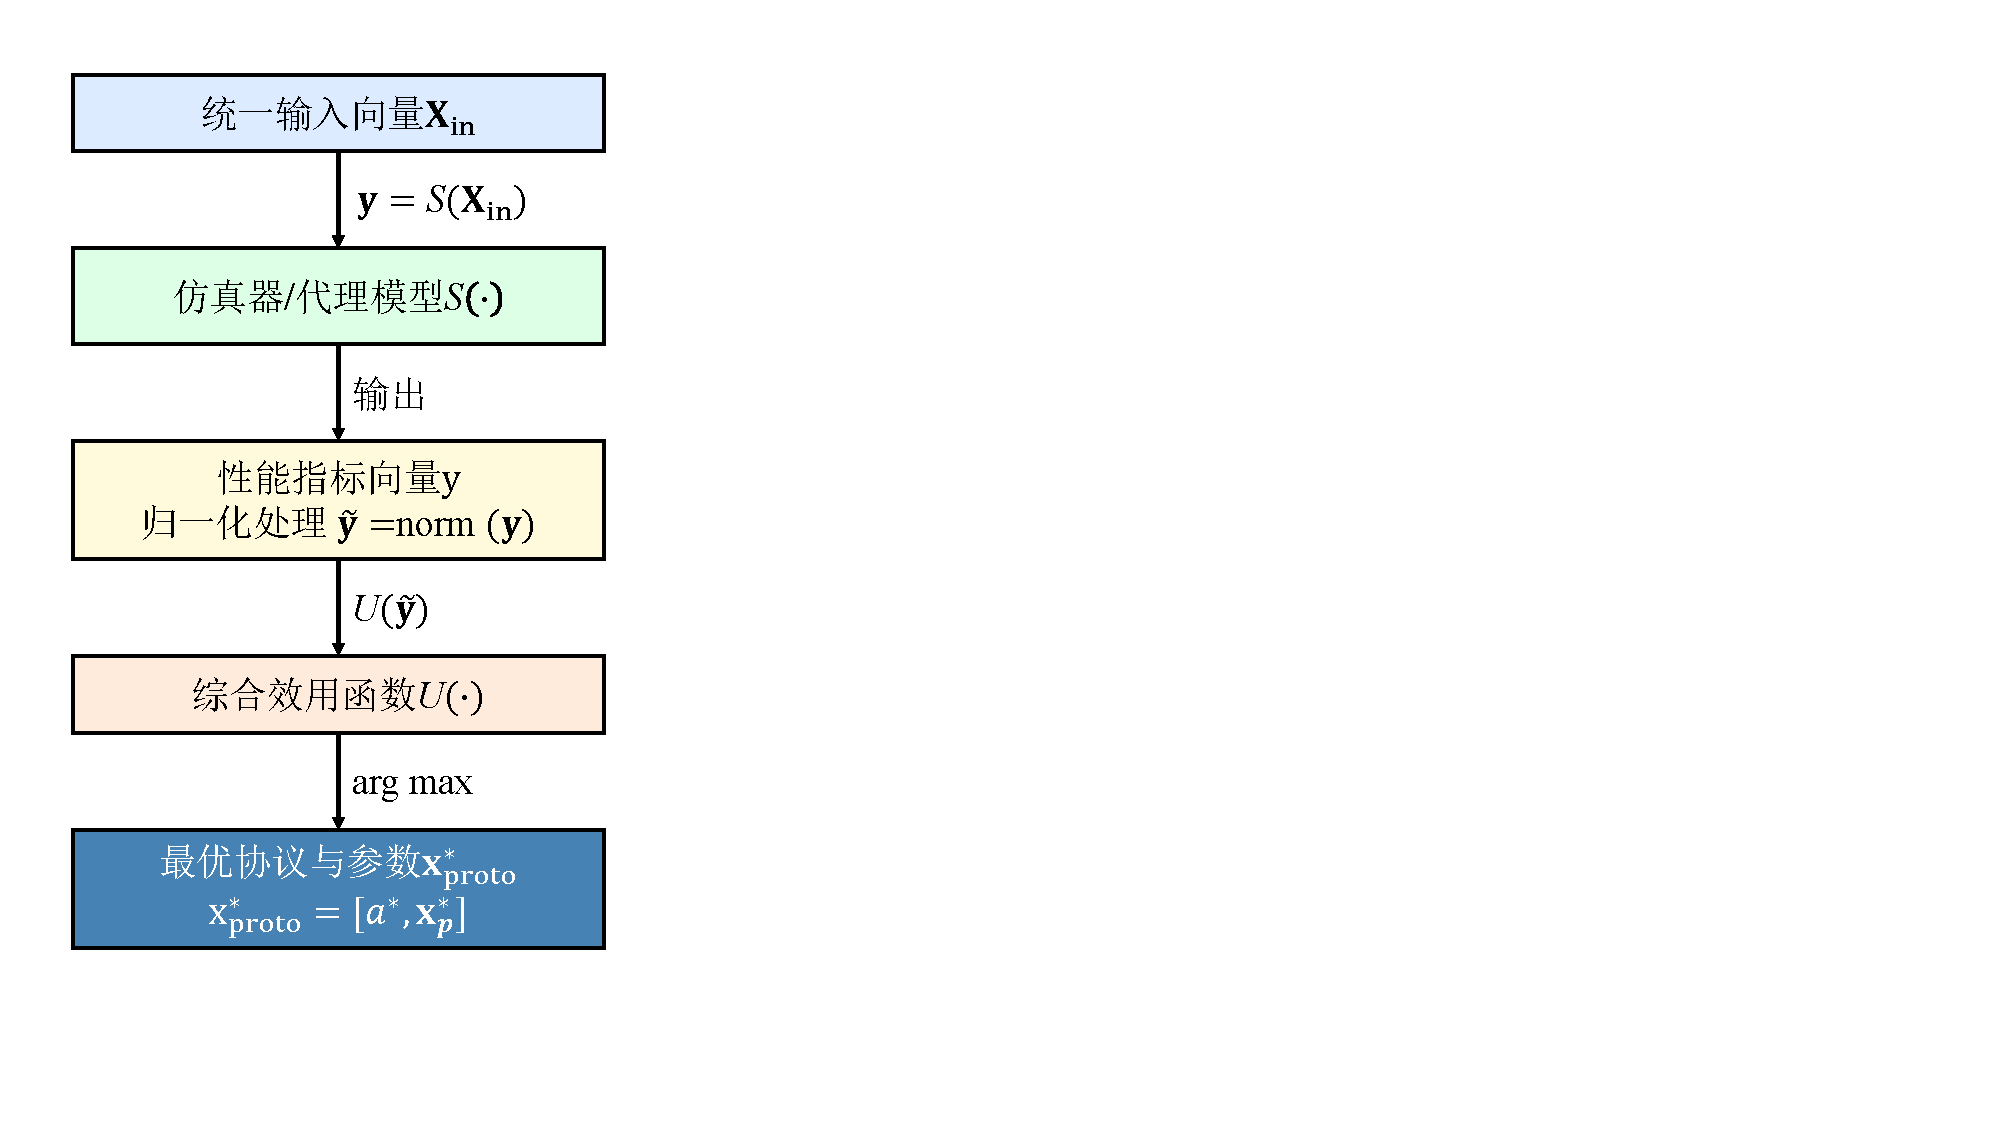
\includegraphics[width=0.5\textwidth]{figure/chap5/model1.pdf}
\caption{统一接入框架与协议选择流程}
\label{fig:chap5_framework}
\end{figure}


\subsection{输入特征标准化与统一接口}
为实现式~\eqref{eq:chap5_overview} 所需的输入表达，本小节给出统一输入 $\mathbf{X}_{\mathrm{in}}$ 的可实现构造方法。本文将特征划分为三类：通用网络参数 $\mathbf{x}_{\mathrm{common}}$，业务流量特征参数 $\mathbf{x}_{\text{traffic}}$，以及协议专属参数 $\mathbf{x}_{\mathrm{proto}}$ 及其有效性掩码 $\mathbf{m}$。

对于通用网络参数 $\mathbf{x}_{\mathrm{common}}$，将其定义为包含网络规模与仿真配置的向量：
$\mathbf{x}_{\mathrm{common}} = [n,\ T]^{\top}$,
其中 $n \in \mathbb{N}^+$ 表示网络节点总数，$T \in \mathbb{N}^+$ 表示仿真或观测的时隙总数。上述参数既用于构建仿真场景，也作为后续学习模型的输入特征，共同刻画系统的整体运行条件。

对于业务流量特征 $\mathbf{x}_{\text{traffic}}$，为准确刻画业务到达的多尺度时空统计特性，本文从网络层与节点层两个层级，分别提取负载强度、突发性与周期性三类特征。具体地，定义五维流量特征向量 $\mathbf{x}_{\text{traffic}} = [\hat{\lambda},\ \mathrm{BI}_{\mathrm{net}},\ \mathrm{BI}_{\mathrm{node}},\ \Psi_{\mathrm{net}},\ \Psi_{\mathrm{node}}]^{\top}$。

设到达矩阵 $\mathbf{A} \in \{0,1\}^{n \times T}$，其中 $A_{i,t}$ 表示节点 $i$ 在时隙 $t$ 是否有包到达。记网络聚合到达序列为 $X(t) = \sum_{i=1}^{n} A_{i,t}$，节点 $i$ 的到达时刻集合为 $\mathcal{T}_i = \{t : A_{i,t} = 1\}$，到达间隔序列为 $\{\Delta t_i^{(k)}\}$，其中 $\Delta t_i^{(k)}$ 为节点 $i$ 第 $k$ 次与第 $k+1$ 次到达的时间间隔。基于此，五维特征定义如下：

\begin{enumerate}[leftmargin=*]
	\item \textbf{归一化网络平均到达率 $\hat{\lambda}$}：表征系统整体流量强度，定义为网络聚合到达序列的单位节点归一化时间平均值 $\hat{\lambda} = \frac{1}{nT} \sum_{t=1}^{T} X(t) = \frac{1}{nT} \sum_{t=1}^{T} \sum_{i=1}^{n} A_{i,t}$。特征 $\hat{\lambda} \in [0, 1]$ 反映了系统的平均活跃节点占比，是区分低流量强度、适中流量强度与拥塞情形的核心指标。
	
	\item \textbf{网络突发度指标 $\mathrm{BI}_{\mathrm{net}}$}：基于网络聚合流量的离散指数（Index of Dispersion）定义。记 $\mu_X = \mathbb{E}[X(t)]$，$\sigma_X^2 = \mathrm{Var}(X(t))$，则离散指数为 $\mathrm{ID}_{\mathrm{net}} = \frac{\sigma_X^2}{\mu_X}$。为将其归一化至 $(-1, 1)$ 区间，定义突发度指标为 $\mathrm{BI}_{\mathrm{net}} = \frac{\mathrm{ID}_{\mathrm{net}} - 1}{\mathrm{ID}_{\mathrm{net}} + 1}$。当 $\mathrm{BI}_{\mathrm{net}} \approx 0$ 时，流量接近泊松分布；$\mathrm{BI}_{\mathrm{net}} > 0$ 表示流量具有强突发性；$\mathrm{BI}_{\mathrm{net}} < 0$ 则表示流量呈现周期性或规则结构。
	
	\item \textbf{节点突发度指标 $\mathrm{BI}_{\mathrm{node}}$}：基于节点到达间隔的变异系数刻画单节点突发性。对节点 $i$，定义其到达间隔的变异系数为 $\mathrm{CV}_i = \frac{\sqrt{\mathrm{Var}(\Delta t_i)}}{\mathbb{E}[\Delta t_i]}$，其中 $\mathbb{E}[\Delta t_i]$ 与 $\mathrm{Var}(\Delta t_i)$ 分别为节点 $i$ 到达间隔的均值与方差。对所有节点的变异系数取平均后归一化：$\mathrm{BI}_{\mathrm{node}} = \frac{\overline{\mathrm{CV}} - 1}{\overline{\mathrm{CV}} + 1}$，其中 $\overline{\mathrm{CV}} = \frac{1}{n} \sum_{i=1}^{n} \mathrm{CV}_i$。特征 $\mathrm{BI}_{\mathrm{node}} \in (-1, 1)$ 反映了节点级流量的突发程度，数值越大表示节点到达越不规则。
	
	\item \textbf{网络周期性强度 $\Psi_{\mathrm{net}}$}：通过网络聚合到达序列 $X(t)$ 的自相关函数度量周期性。记去均值后的序列为 $\tilde{X}(t) = X(t) - \mu_X$，自相关函数为 $R(\tau) = \frac{1}{T} \sum_{t=1}^{T-\tau} \tilde{X}(t) \tilde{X}(t+\tau)$。定义周期性强度为最大归一化自相关值：$\Psi_{\mathrm{net}} = \max_{1 \le \tau \le \tau_{\max}} \frac{R(\tau)}{R(0)}$，其中 $\tau_{\max}$ 为最大检测周期长度。特征 $\Psi_{\mathrm{net}} \in [0, 1]$，数值越大表示网络流量的周期性越强。
	
	\item \textbf{节点周期性强度 $\Psi_{\mathrm{node}}$}：基于节点到达间隔的归一化变异系数刻画单节点周期性。该指标利用到达间隔的相对变异程度度量其规则性：当到达间隔方差相对于均值平方的比值越小时，到达模式越接近确定性周期过程。对节点 $i$，定义其周期性指标为 $P_i = \max\left(0,\ 1 - \frac{\mathrm{Var}(\Delta t_i)}{\left(\mathbb{E}[\Delta t_i]\right)^2}\right)$，其中 $\frac{\mathrm{Var}(\Delta t_i)}{\left(\mathbb{E}[\Delta t_i]\right)^2}$ 为归一化变异系数的平方。对全部节点的周期性指标取算术平均，得到节点层周期性强度：$\Psi_{\mathrm{node}} = \frac{1}{n} \sum_{i=1}^{n} P_i$。特征 $\Psi_{\mathrm{node}} \in [0, 1]$，数值越大表示节点到达间隔越规则，周期性越强。
\end{enumerate}

对于协议专属参数 $\mathbf{x}_{\mathrm{proto}}$ 及有效性掩码 $\mathbf{m}$，本文采用统一参数超集与掩码的表示方案，以在多协议共存场景下建立统一的输入接口。设候选接入协议集合为 $\mathcal{P} = \{a_1, a_2, \ldots, a_6\}$，包括 SA、SAST、CBA、RSA、CRDSA 及 IRSA。每一种协议 $a \in \mathcal{P}$ 对应一组可调参数集合 $\mathcal{X}_p$。
为消除因协议参数维度不一致而产生的维度非对齐问题，本文将候选协议集合中所有参数的并集统一放入一个高维参数向量 $\mathbf{x}_{\mathrm{proto}} \in \mathbb{R}^{d_{\max}}$，其中 $d_{\max} = 1 + \max_{a  \in \mathcal{P}} |\mathcal{X}_p|$ 为统一向量维度，包含协议标识符及所有协议参数的超集。该向量的第一个分量为协议类型标识符 $a \in \mathcal{P}$，其余分量包含接入概率 $q$、连续传输长度 $M$、副本/重传次数 $L$、帧长度 $T_{\mathrm{frame}}$ 等所有可能的协议参数；当某一协议不涉及其中部分参数时，对应维度仍保留作为占位符。统一参数向量的完整形式为：
$\mathbf{x}_{\mathrm{proto}} = [a, q,\ M,\ L,\ T_{\mathrm{frame}},\ \ldots]^{\top}$, 
其中省略号对应除列示参数外的其余占位分量。

为严格刻画占位参数在当前协议下的有效性，引入与 $\mathbf{x}_{\mathrm{proto}}$ 同维的二值掩码向量 $\mathbf{m} \in \{0,1\}^{d_{\max}}$。掩码的具体应用将在后续的数据采样阶段详细阐述。在预处理与模型输入阶段，对应掩码为零的参数分量通过元素级乘积 $\mathbf{x}_{\mathrm{proto}} \odot \mathbf{m}$ 被统一置零或屏蔽，从而在保留统一维度表示的同时，防止无效参数对后续学习与优化过程造成干扰。输入特征与性能指标的摘要见表~\ref{tab:input_features}。
最终与前文一致，完整标准化输入向量表示为
\begin{equation}
\mathbf{X}_{\mathrm{in}} = \big[\mathbf{x}_{\text{traffic}},\ \mathbf{x}_{\mathrm{common}},\ \mathbf{x}_{\mathrm{proto}},\ \mathbf{m}\big].
\end{equation}


\begin{table}[t]
	\centering
	\caption{标准化输入与性能指标摘要}
	\label{tab:input_features}
	\renewcommand{\arraystretch}{1.2}
	\begin{tabular}{@{}l l p{9cm}@{}}
	\toprule
		特征组 & 符号 & 含义 / 备注 \\
		\midrule
		$\mathbf{x}_{\text{traffic}}$ & $\hat{\lambda}$ & 归一化网络平均到达率，范围 $[0, 1]$。\\
		& $\mathrm{BI}_{\mathrm{net}}$ & 网络突发度指标，范围 $(-1,1)$。\\
		& $\mathrm{BI}_{\mathrm{node}}$ & 节点突发度指标，范围 $(-1,1)$。\\
		& $\Psi_{\mathrm{net}}$ & 网络周期性强度，范围 $[0,1]$。\\
		& $\Psi_{\mathrm{node}}$ & 节点周期性强度，范围 $[0,1]$。\\
		\midrule
		$\mathbf{x}_{\mathrm{common}}$ & $n$ & 节点数量。\\
		& $T$ & 时隙数量。\\
		\midrule
		$\mathbf{x}_{\mathrm{proto}}$ & $a$ & 协议类型标识，$a\in\mathcal{P}$（向量第一个分量）。\\
		& $q$ & 接入概率。\\
		& $M$ & 连续传输长度。\\
		& $L$ & 副本/重传次数。\\
		& $T_{\mathrm{frame}}$ & 帧长度。\\
		& $\ldots$ & 其他协议参数（后续会补全zzzwl）。\\
		\midrule
		$\mathbf{m}$ & $m_k$ & 有效性掩码：$m_k=1$ 若第 $k$ 个协议参数在当前协议下有效，否则为 $0$。\\
		\midrule
		$\mathbf{y}$ & $\lambda_{\mathrm{out}}$ & 吞吐量。\\
		& $D$ & 平均时延。\\
		& $J_T$ & 公平性。采用 Jain 指数并做归一化。\\
		& $C_{\mathrm{rx}}$ & 接收端计算负荷。\\
		& $I_{\mathrm{impl}}$ & 协议实现复杂度。\\
		\bottomrule
	\end{tabular}
\end{table}

\subsection{统一仿真映射与效用构造}

在统一输入接口 $\mathbf{X}_{\mathrm{in}}$ 确定后，需要进一步给出从输入到性能度量的可复现映射。为此，本文构建统一的离散事件仿真映射$S(\cdot)$：其输入为统一输入向量 $\mathbf{X}_{\mathrm{in}}$，仿真器据此生成对应网络场景并执行随机接入过程，最终输出性能—资源指标向量
\begin{equation}
	\mathbf{y}=S\!\left(\mathbf{X}_{\mathrm{in}}\right)
	=\big[\lambda_{\mathrm{out}},\ D,\ J_T,\ C_{\mathrm{rx}},\ I_{\mathrm{impl}}\big],
\end{equation}
其中 $\lambda_{\mathrm{out}}$ 表示系统吞吐量，$D$ 表示平均数据包时延，$J_T$ 表示公平性（采用 Jain 指数刻画），$C_{\mathrm{rx}}$ 表示接收端计算负荷，$I_{\mathrm{impl}}$ 表示协议实现复杂度。上述指标集合兼顾业务性能与实现代价，便于在多协议、多参数配置下进行统一评估与对比。

为消除不同指标量纲与数值尺度差异对比较与决策造成的影响，并保证跨协议评估的一致性，本文在同一对比组内对各维指标采用最小最大归一化，并将所有指标统一转换为效用型指标。记第 $k$ 个指标 $y_k$ 在对比组内的取值范围为 $[y_k^{\min}, y_k^{\max}]$，则归一化后的指标 $\tilde{y}_k$ 定义为
\begin{equation}
	\tilde{y}_k =
	\begin{cases}
	\dfrac{y_k-y_k^{\min}}{y_k^{\max}-y_k^{\min}}, & y_k \ \text{为效用型指标},\\[10pt]
	1-\dfrac{y_k-y_k^{\min}}{y_k^{\max}-y_k^{\min}}, & y_k \ \text{为成本型指标},
	\end{cases}
\end{equation}
其中效用型指标是指数值增大表示性能提升的指标，如吞吐量 $\lambda_{\mathrm{out}}$ 和公平性 $J_T$；成本型指标是指数值减小表示性能改善的指标，如时延 $D$ 与计算负荷 $C_{\mathrm{rx}}$。该归一化方法将所有指标映射至 $[0,1]$ 区间，并保证归一化后的指标均满足数值越大性能越优的单调关系。由此得到归一化指标向量
\begin{equation}
	\tilde{\mathbf{y}}=\mathrm{norm}(\mathbf{y})
	=\big[\tilde{\lambda}_{\mathrm{out}},\ \tilde{D},\ \tilde{J}_T,\ \tilde{C}_{\mathrm{rx}},\ \tilde{I}_{\mathrm{impl}}\big].
\end{equation}

在此基础上，为将多维指标映射为单一可优化目标，本文采用加权线性综合效用函数
\begin{equation}
	U\big(\tilde{\mathbf{y}}\big)=
	w_{\lambda}\tilde{\lambda}_{\mathrm{out}}
	+w_{D}\tilde{D}
	+w_{J}\tilde{J}_T
	+w_{C}\tilde{C}_{\mathrm{rx}}
	+w_{I}\tilde{I}_{\mathrm{impl}},
\end{equation}
其中 $w_i\ge 0$ 且 $\sum_i w_i=1$。权重向量 $\{w_i\}$ 用于表征业务对吞吐、时延、公平性以及资源/复杂度代价的偏好，可依据应用需求设定；同时，可通过改变权重进行敏感性分析，以检验联合选择结论的稳健性。

%\paragraph{资源约束下的协议与参数联合优化}
\subsection{等价重写：资源约束下的联合优化形式}
为便于后续代理模型训练与快速优化算法中目标计算、约束检查与可行域投影的统一实现，本节将式~\eqref{eq:chap5_overview} 所述问题改写为标准约束优化形式。该表述与原问题在决策变量、优化目标及约束条件上完全等价，区别仅在于将隐式关系显式展开，以适配标准优化求解器的输入要求。

优化问题的标准形式表述如下：
\begin{equation}\label{eq:chap5_constrained}
	\begin{aligned}
		\max_{\,\mathbf{x}_{\mathrm{proto}}}\quad 
		& U\big( \tilde{\mathbf{y}} \big) \\[6pt]
		\text{s.t.}\quad
		& \mathbf{X}_{\mathrm{in}}=\big[\mathbf{x}_{\text{traffic}},\ \mathbf{x}_{\mathrm{common}},\ \mathbf{x}_{\mathrm{proto}},\ \mathbf{m}\big],\\[3pt]
		& \tilde{\mathbf{y}} = \mathrm{norm}\!\left(\mathbf{y}\right),\ \mathbf{y} = S\!\left( \mathbf{X}_{\mathrm{in}} \right), \\[4pt]
		& C_{\mathrm{rx}}\big(\mathbf{x}_{\mathrm{proto}}\big) \le C_{\max},\\[3pt]
		& I_{\mathrm{impl}}(\mathbf{x}_{\mathrm{proto}}[1]) \le I_{\max}.
	\end{aligned}
\end{equation}

式~\eqref{eq:chap5_constrained} 的决策变量为统一参数向量 $\mathbf{x}_{\mathrm{proto}}$，其第一个分量 $\mathbf{x}_{\mathrm{proto}}[1]$ 为协议标识符，其余分量为各协议参数。决策变量需满足所选协议的合法参数空间约束，通过掩码 $\mathbf{m}$ 界定有效参数维度。第一行约束显式构建统一输入向量，第二行约束定义从输入到归一化性能指标的映射关系。第三、四行约束分别限定接收端计算负荷与协议实现复杂度不超过系统资源阈值 $C_{\max}$ 与 $I_{\max}$。

可以看到，该优化问题的解为满足全部约束的最优统一参数向量 $\mathbf{x}_{\mathrm{proto}}^*$，其中包含了最优协议类型及其对应参数。


% =========================================================
% 第 5.2 节：仿真数据生成与性能分析
% =========================================================

\section{基于离散事件仿真的接入协议数据集构建与仿真结果分析}
\label{sec:simulation_data}

为训练能够准确预测不同协议配置下网络性能的代理模型，需要构建高质量的训练数据集。本节首先阐述参数空间的采样策略，随后在\ref{subsec:unified_simulator}小节介绍统一仿真器 $S(\cdot)$ 的设计与实现，接着详细说明基于仿真器的数据集生成流程，最后通过可视化分析展示不同协议在典型场景下的性能差异，为后续代理模型的构建提供数据基础与性能基准。

\subsection{两阶段参数空间采样策略}
\label{subsec:grid_sampling}

训练数据的质量与参数空间覆盖率直接影响后续代理模型的预测精度。本小节需要在由业务流量特征参数 $\mathbf{x}_{\text{traffic}}$ 与协议专属参数 $\mathbf{x}_{\mathrm{proto}}$ 共同构成的混合参数空间内生成样本。为便于组织采样与对比评估，本文将该混合空间分解为三个相互独立但在实验配置中联合遍历的维度，即流量强度维度、流量形态维度与协议参数维度。其中，流量强度维度由归一化网络平均到达率 $\hat{\lambda}$ 表征，用于刻画系统所处的低流量强度、中等流量强度与拥塞状态；流量形态维度用于刻画在相同平均流量强度下到达过程的统计差异；协议参数维度用于描述不同协议机制下的关键控制参数组合。基于上述分解可以看出，若在三维联合空间上直接采用单一粒度的均匀网格进行采样，一方面会在性能变化相对平缓的区域产生大量冗余样本，另一方面又容易在性能转折与峰值附近等关键区域出现采样不足，从而削弱后续代理模型对关键决策边界与最优工作点邻域的刻画能力。为在控制样本总量的同时兼顾全局覆盖与局部精度，本文对流量强度维度与协议参数维度采用两阶段自适应采样策略；与之相对，流量形态维度采用固定离散场景集合并在两个阶段中保持一致遍历，以构造可控对比基座并保证跨协议样本的可比性。具体而言，每一条样本由一组协议参数配置与一个流量强度取值共同确定，并在预先固定的流量形态场景集合下分别生成到达序列与性能标签，第一阶段用于快速获得性能曲线的整体轮廓并定位关键工作区间，第二阶段在关键区间内加密采样以刻画转折与峰值邻域的细粒度变化。

在流量形态维度上，本文以离散场景集合的方式给出典型到达过程。具体而言，本文考虑三类典型业务流量场景。场景一为均匀到达，用于模拟节点独立随机到达，常见于大规模传感器网络分散采集，其流量特征为 $\mathrm{BI}_{\mathrm{net}} \approx 0$ 且 $\Psi_{\mathrm{net}} \approx 0$，对应近似泊松到达过程。场景二为突发到达，用于刻画事件驱动型应用的集中上报特性，通过批量到达过程建模，其流量特征为 $\mathrm{BI}_{\mathrm{net}} \in [0.3, 0.7]$ 且 $\Psi_{\mathrm{net}} \in [0, 0.2]$，表征中等至强突发性。场景三为周期到达，用于模拟周期性传感采样或时隙同步传输，其流量特征为 $\mathrm{BI}_{\mathrm{net}} \in [-0.5, -0.2]$ 且 $\Psi_{\mathrm{net}} \in [0.6, 0.9]$，体现规则周期结构。后续采样过程中，对于每一个流量强度取值与每一组协议参数配置，均在上述三类流量形态下分别生成样本，从而在平均流量强度一致的条件下对不同到达过程差异进行可控对比。



% ...existing code...

% ...existing code...



\textbf{第一阶段：粗粒度均匀采样。}
第一阶段旨在以较少样本量快速覆盖参数空间全域，识别各协议的性能分布特征。对于业务流量特征参数 $\mathbf{x}_{\text{traffic}}$，其核心参数归一化网络平均到达率 $\hat{\lambda}$ 需根据各协议的理论性能上界设定合理的采样范围。值得注意的是，\textbf{不同随机接入协议的理论容量与有效工作范围存在显著差异}，这直接决定了其适用的流量强度区间。例如，经典Slotted ALOHA（SA）协议的理论最大吞吐量为 $1/e \approx 0.368$，对应的有效到达率通常限制在 $0.5$ 以内；SAST协议通过连续传输机制将理论最大吞吐提升至约0.5，有效范围扩展至 $0.7$ 左右；而基于连续干扰消除（SIC）的CRDSA/IRSA协议则可在显著更高的负载水平（$\hat{\lambda} > 0.55$）下保持较好的性能。

若对所有协议采用统一的宽泛采样范围（如 $\hat{\lambda} \in [0, 1]$），将导致以下严重的采样偏差问题：低容量协议（如SA）的绝大多数样本会落入其性能已饱和或甚至退化的超容量区域，这些样本对学习真实性能曲线形态无实质帮助；相反，对于高容量协议，用于描述其真正工作区间（通常位于中等至高负载）的样本会严重不足，导致代理模型在这些关键工作点的预测精度下降。为此，本文根据各协议的理论吞吐上界与实际有效工作范围，为每种协议精心设计了差异化的 $\hat{\lambda}$ 采样区间，确保每种协议的样本都集中在其实际可工作的负载区域内。
具体而言，对于归一化网络平均到达率 $\hat{\lambda}$，各协议的粗采样范围设定如下：
\begin{itemize}[leftmargin=*]
	\item SA协议：$\hat{\lambda} \in [0.01, 0.5]$，步长 $\Delta\hat{\lambda} = 0.05$，约10个采样点；
	\item SAST、CBA协议：$\hat{\lambda} \in [0.01, 0.7]$，步长 $\Delta\hat{\lambda} = 0.05$，约13个采样点；
	\item RSA协议：$\hat{\lambda} \in [0.01, 0.2]$，步长 $\Delta\hat{\lambda} = 0.05$，约15个采样点；
	\item CRDSA、IRSA协议：$\hat{\lambda} \in [0.01, 0.8]$，步长 $\Delta\hat{\lambda} = 0.05$，约21个采样点。
\end{itemize}

对于每一个 $\hat{\lambda}$ 的粗采样点，流量生成模块分别在上述三类流量形态场景下生成到达序列，从而在相同平均流量强度条件下对不同到达过程差异进行对比评估。尽管三类场景的归一化网络平均到达率相同，但流量特征向量 $\mathbf{x}_{\text{traffic}}$ 的其他分量存在显著差异，进而导致协议性能表现产生差异。

对于协议专属参数 $\mathbf{x}_{\mathrm{proto}}$ 的采样，本文采用分协议定制化策略。每种协议具有不同的有效参数集合 $\mathcal{X}_a$，其中包含连续型与离散型参数。对于\textbf{连续型协议参数}（如接入概率 $q$），在其有效范围内均匀设置若干采样点；对于\textbf{离散型协议参数}（如副本数 $L$、重传次数 $M$、帧长度 $T_{\mathrm{frame}}$等），则遍历其所有实际可行的典型取值。例如，副本数 $L$ 通常设置 $\{2, 3, 4 \}$ 四个值，帧长度 $T_{\mathrm{frame}}$ 设置 $\{10, 20, 30\}$ 三个值。协议参数的笛卡尔积生成该协议的参数配置空间。

通过对协议类型、归一化网络平均到达率、业务流量场景以及协议专属参数的全面组合，生成第一阶段的粗采样配置集合。对于每种协议，采样点数由协议的到达率采样数、3种业务流量场景，以及各协议参数的采样点数共同决定。这样的组合方式确保了数据集不仅覆盖了协议与参数的多样性，还确保了对不同流量模式的全面刻画。
对粗采样配置中的每组参数组合，通过统一仿真器 $S(\cdot)$ 评估其性能指标。基于粗采样结果，可以初步识别各协议在不同业务流量场景与到达率组合下的性能规律，尤其是吞吐量在特定场景下的峰值位置。

\textbf{第二阶段：峰值区域细采样。}
第二阶段针对粗采样结果中识别出的性能关键区域进行加密采样，以捕捉性能曲线的精细变化特征。具体而言，对于每种协议，分析其粗采样得到的吞吐量曲线，识别峰值吞吐量对应的到达率区间。以SAST协议为例，若粗采样显示其峰值吞吐出现在约0.5（包/时隙）的到达率处，则在该值附近（如区间0.45-0.55）以更细的步长进行二次采样，额外生成十几到二十多个样本点。

细采样不仅针对业务流量到达率参数，还需要扩展至协议专属参数。例如对于SA协议，在性能转折区域需要进行对协议参数进行加密采样。第二阶段的样本规模根据各协议峰值区域的范围而定，每种协议需要额外增加数百到千级别的样本点。

将两阶段采样得到的所有样本合并，构成完整的训练数据集。由于峰值区域的样本密度更高，代理模型在训练过程中将对关键性能区域获得更强的拟合能力，从而在实际应用中能够更准确地预测最优工作点附近的性能表现。总体来看，通过两阶段采样策略相比均匀细采样可显著节省样本量，同时显著提升了数据集在性能关键区域的代表性。

\subsection{统一仿真器的设计与实现}
\label{subsec:unified_simulator}

统一仿真器 $S(\cdot)$ 是连接输入配置与性能指标的核心映射模块，其设计需同时满足多协议支持、精确性与可扩展性要求。本文基于离散事件仿真框架采用模块化设计实现该仿真器，通过各模块的协调完成对六种随机接入协议的统一建模与性能评估。

统一仿真器采用分层模块化架构，包含以下核心组件：

\begin{itemize}[leftmargin=*]
	\item \textbf{配置解析模块}：解析统一输入向量 $\mathbf{X}_{\mathrm{in}}$，提取网络参数 $\mathbf{x}_{\text{common}}$（节点数 $n$、时隙数 $T$）、流量类型标识 $\text{traffic\_type}$(该标识需要自定义)、流量特征向量 $\mathbf{x}_{\text{traffic}}$（仅包含$\hat{\lambda}$）以及协议专属参数向量 $\mathbf{x}_{\mathrm{proto}}$（其首个分量为协议类型标识 $a$，其余分量为协议参数）。

	\item \textbf{流量生成和特征提取模块}：依据流量类型标识 $\text{traffic\_type}$ 选择到达过程模型（均匀到达采用泊松过程、突发到达采用Markov调制泊松过程、周期到达采用确定性周期同步，这些生成过程会预设生成参数），并在给定平均到达率 $\hat{\lambda}$ 下为各节点按时隙生成到达包序列。由于生成参数固定，得到的流量序列仅覆盖有限组预定义的突发强度与周期强度，从而保证不同实验配置间的可复现性。基于生成的到达包序列，计算并输出 $\mathbf{x}_{\text{traffic}}$ 中除 $\hat{\lambda}$ 外的其余特征指标 $\mathrm{BI}_{\mathrm{net}}$、$\mathrm{BI}_{\mathrm{node}}$、$\Psi_{\mathrm{net}}$ 和 $\Psi_{\mathrm{node}}$。

	\item \textbf{协议执行与仿真模块}：协议策略由协议专属参数向量 $\mathbf{x}_{\mathrm{proto}}$ 参数化，其中其首个分量确定协议类型 $a$。具体而言，协议类型 $a$ 对应协议执行引擎，$\mathbf{x}_{\mathrm{proto}}$ 剩余分量则对应一组参数化的协议策略。仿真器在仿真前先初始化到正确的协议执行引擎，并在每个时隙依据该策略完成发送决策、副本生成与队列状态更新；同时与信道仿真子模块协同完成并行发送的冲突检测。对支持SIC的协议（CRDSA/IRSA），进一步调用解码器执行帧级连续干扰消除迭代解码，并统计接收端计算负荷 $C_{\mathrm{rx}}$。协议执行引擎会对各协议的关键机制进行封装，具体如下：
	\begin{itemize}[leftmargin=*, itemsep=0.2em]
		\item \textbf{SA}：时隙ALOHA，节点在有包时以固定接入概率 $q$ 发送。
		\item \textbf{SAST}：连续传输时隙ALOHA，若上一时隙成功则接入概率置1连续发送，否则回到概率发送。
		\item \textbf{CBA}：基于连接的Aloha，以固定概率$q$建立连接，连接成功后会无竞争发送$M$个包。
		\item \textbf{RSA}：分帧结构，帧内先预约后传输，两阶段等长；节点在预约时隙竞争信道，预约成功的节点在对应数据时隙无竞争发送。
		\item \textbf{CRDSA}：分帧结构，每包生成固定 $L$ 个副本随机分布在帧内各时隙，接收端利用SIC在帧级迭代消除碰撞。
		\item \textbf{IRSA}：分帧结构，副本数 $L$ 由预设度分布采样，结合SIC在帧级迭代解码以提升成功概率。
	\end{itemize}

	\item \textbf{性能统计模块}：实时记录成功发送包数、累计时延、各节点吞吐、SIC解码次数等统计量，在仿真完成后计算最终的吞吐量 $\lambda_{\mathrm{out}}$、平均时延 $D$、公平性指数 $J_T$、计算负荷 $C_{\mathrm{rx}}$ 及实现复杂度 $I_{\mathrm{impl}}$。
\end{itemize}

上述模块通过统一接口在离散事件仿真框架下协同运行，从而实现对多协议、多参数配置的统一评估。下面给出统一仿真器的核心实现流程，其执行流程遵循初始化、时隙迭代与结果汇总三个阶段：

\begin{algorithm}[htbp]
	\caption{统一仿真器执行流程}
	\label{alg:unified_simulator_main}
	\KwIn{配置参数 $\mathbf{X}_{\text{in}} = (\mathbf{x}_{\mathrm{common}}, \mathbf{x}_{\text{traffic}}(\text{部分占位}), \mathbf{x}_{\mathrm{proto}})$，\text{traffic\_type} } 
	\KwOut{性能指标 $\mathbf{y} = [\lambda_{\mathrm{out}}, D, J_T, C_{\mathrm{rx}}, I_{\mathrm{impl}}]^{\top}$}
	
	配置解析模块：$n, T, \text{traffic\_type}, \hat{\lambda}, \mathbf{x}_{\mathrm{proto}} \leftarrow \text{Parse}(\mathbf{X}_{\text{in}})$\\
	协议标识提取：$a \leftarrow \mathbf{x}_{\mathrm{proto}}[1]$\\
	系统初始化：创建 $n$ 个节点的缓冲队列、信道状态记录、事件队列\\
	流量生成与特征提取：基于 $\text{traffic\_type}$ 和归一化网络平均到达率 $\hat{\lambda}$ 选择到达过程（参数预设），生成到达矩阵 $\mathbf{A}\in\{0,1\}^{n\times T}$，并计算更新 $\mathrm{BI}_{\mathrm{net}}$、$\mathrm{BI}_{\mathrm{node}}$、$\Psi_{\mathrm{net}}$、$\Psi_{\mathrm{node}}$\\
	加载协议引擎以及参数：根据$a$加载协议执行引擎，根据$\mathbf{x}_{\mathrm{proto}}$加载协议策略\\

	性能统计初始化：$\text{success\_counter} \leftarrow 0, \text{delay\_counter} \leftarrow 0$ 等\\
	\For{$t = 1$ \textbf{to} $T$}{
        1. 到达生成：由到达矩阵$\mathbf{A}\in\{0,1\}^{n\times T}$确定各节点的包入队情况\;
        
        2. 接入/副本策略：根据协议规则与协议参数生成发送集合（或本帧内的副本布局/预约选择）\;
        
        3. 信道解析：执行信道判决，得到并行发送导致的成功/冲突结果（帧结构协议会形成帧内碰撞图）\;
        
        4. 若协议支持帧级 SIC，累计接收端计算量与解码次数\;
        
        5. 根据成功结果更新队列/协议内部状态，并更新统计量\;
	}
	计算吞吐量：$\lambda_{\mathrm{out}} \leftarrow \text{success\_counter} / T$\\
	计算平均时延：$D \leftarrow \text{sum\_delay} / \text{success\_counter}$\\
	计算公平性指数：$J_T \leftarrow \text{Jain}(\text{node\_throughputs})$\\
	计算实现复杂度：$I_{\mathrm{impl}} \leftarrow \text{Complexity}(\mathbf{x}_{\mathrm{proto}}[1], \mathbf{x}_{\mathrm{proto}})$\\
	组织输出：$\mathbf{y} \leftarrow [\lambda_{\mathrm{out}}, D, J_T, \text{mean}(C_{\mathrm{rx}}), I_{\mathrm{impl}}]^{\top}$\\
	\Return $\mathbf{y}$
\end{algorithm}

\begin{table}[htbp]
	\centering
	\caption{统一仿真器关键参数汇总}
	\label{tab:simulator_params}
	\renewcommand{\arraystretch}{1.2}
	\begin{tabular}{llll}
		\toprule
		\textbf{参数类别} & \textbf{符号} & \textbf{典型值/范围} & \textbf{说明} \\
		\midrule
		\multirow{4}{*}{基本参数} 
		& $n$ & 100 & 网络节点数 \\
		& $T$ & $3 \times 10^5$ & 仿真时隙数 \\
		& $\text{traffic\_type}$ & \{U, B, P\} & 流量类型：均匀(U)、突发(B)、周期(P) \\
		& $\hat{\lambda}$ & $[0.001, 0.8]$ & 归一化网络平均到达率 \\
		\midrule
		\multirow{2}{*}{SA/SAST 参数} 
		& $q$ & $[0.001, 0.1]$ & 接入概率 \\

		\midrule
		\multirow{2}{*}{CBA 参数} 
		& $q$ & $[0.001, 0.1]$ & 接入概率 \\
		& $M$ & $[5, 20]$ & 连续传输长度 \\
		\midrule
		\multirow{1}{*}{RSA 参数} 
		& $T_{\mathrm{frame}}$ & $[10, 20, 30]$ & 帧长度 \\
		\midrule
		\multirow{3}{*}{CRDSA 参数} 
		& $L$ & $\{2, 3, 4\}$ & 副本数 \\
		& $T_{\mathrm{frame}}$ & $[10, 20, 30]$ & 帧长度 \\
		& $I_{\mathrm{sic}}^{\max}$ & $\{10, 20\}$ & SIC最大迭代次数 \\
		\midrule
		\multirow{3}{*}{IRSA 参数} 
		& $\Gamma$ & \{A3, A4\} & 副本数度分布 \\
		& $T_{\mathrm{frame}}$ & $[10, 20, 30]$ & 帧长度 \\
		& $I_{\mathrm{sic}}^{\max}$ & $\{10, 20\}$ & SIC最大迭代次数 \\
		\bottomrule
	\end{tabular}
\end{table}
通过上述设计，统一仿真器能够高效、准确地评估不同协议配置下的网络性能，为数据集构建提供可靠的性能标签。

\subsection{数据集构建与预处理}
\label{subsec:dataset_construction}

\textcolor{red}{在该小节中的数据，不一定是准确的，后续还要修订，这里仅给出大致叙述逻辑。zzzwl}

基于两阶段采样策略与统一仿真器，本文构建了覆盖六种协议、多种流量强度与参数配置的综合性能数据集。数据集构建过程如下：

\begin{enumerate}[leftmargin=*]
	\item \textbf{采样执行}：对于候选协议集合 $\mathcal{P} = \{\text{SA, SAST, CBA, RSA, CRDSA, IRSA}\}$ 中的每种协议，按照\ref{subsec:grid_sampling}节所述的网格搜索策略生成参数组合。为保证采样配置能够无歧义映射到统一仿真器输入，采样变量与仿真器关键参数一一对应，具体参数名及典型取值范围见表~\ref{tab:simulator_params}。以SA为例，关键参数包括归一化网络平均到达率$\hat{\lambda} \in [0.1, 0.5]$（20个采样点），与接入概率 $q \in [0.001, 0.1]$（20个采样点），共生成 $20 \times 20 = 400$ 组配置。
	
	\item \textbf{仿真执行}：对每组参数配置 $\mathbf{X}_{\text{in}}^{(i)}$，调用统一仿真器执行仿真实验。仿真器在固定网络规模（$n=100$）与仿真时隙数（$T=3 \times 10^5$）下运行，对应表~\ref{tab:simulator_params}中的基本参数配置。为降低随机性影响，每组配置重复运行5次独立实验，取性能指标的平均值作为最终标签 $\mathbf{y}^{(i)}$。
	
	\item \textbf{数据清洗}：剔除仿真失败或出现异常值的样本（如数值溢出、队列发散、解码不收敛等），并对极端异常值进行标记。表~\ref{tab:dataset_summary}中的"采样配置数"与"有效样本数"反映了数据清洗前后的样本统计。各协议最终保留的有效样本数分别为：SA（395）、SAST（782）、CBA（791）、RSA（588）、CRDSA（1156）、IRSA（1432），合计 5144 个有效样本。
	
	\item \textbf{归一化处理}：对连续型特征（如归一化网络平均到达率 $\hat{\lambda}$、接入概率 $q$）保持在其定义域内，流量特征（$\mathrm{BI}_{\mathrm{net}}$、$\mathrm{BI}_{\mathrm{node}}$、$\Psi_{\mathrm{net}}$、$\Psi_{\mathrm{node}}$）已在特征提取时归一化至特定范围；对离散型特征（协议类型、副本数 $L$、帧长度 $T_{\mathrm{frame}}$ 等）采用整数编码或独热编码。性能指标 $\mathbf{y}$ 采用Z-Score标准化，以加速模型训练收敛。
	
	\item \textbf{数据划分}：按照 8:1:1 的比例将数据集划分为训练集（约 4100 样本）、验证集（约 520 样本）与测试集（约 524 样本）。为保证协议类型在三个子集中均衡分布，采用分层随机划分策略，避免数据泄露与类别不平衡问题。
\end{enumerate}

表~\ref{tab:dataset_summary} 总结了最终数据集的统计特性。

\begin{table}[htbp]
	\centering
	\caption{仿真数据集统计摘要}
	\label{tab:dataset_summary}
	\renewcommand{\arraystretch}{1.2}
	\begin{tabular}{lcccc}
	\toprule
		\textbf{协议类型} & \textbf{参数维度} & \textbf{采样配置数} & \textbf{有效样本数} & \textbf{归一化网络平均到达率范围（$\hat{\lambda}$）} \\
	\midrule
		SA & 2 & 400 & 395 & $[0.01, 0.5]$ \\
		SAST & 3 & 800 & 782 & $[0.01, 0.7]$ \\
		CBA & 3 & 800 & 791 & $[0.01, 0.7]$ \\
		RSA & 3 & 600 & 588 & $[0.01, 0.2]$ \\
		CRDSA & 4 & 1200 & 1156 & $[0.01, 0.8]$ \\
		IRSA & 5 & 1500 & 1432 & $[0.01, 0.8]$ \\
	\midrule
		\textbf{总计} & 无 & \textbf{5300} & \textbf{5144} & 无 \\
	\bottomrule
	\end{tabular}
\end{table}

通过上述数据集构建流程，本文获得了覆盖多协议、多参数配置与多种流量形态的仿真样本库。需要强调的是，数据集中的性能标签由统一仿真器在统一网络规模与统一统计口径下生成，且两阶段采样保证了各协议在其有效工作区间内具有足够的样本密度。因此，该数据集不仅用于后续代理模型训练，同时也可作为可复现的性能基准来源。基于此，下一小节将在不额外引入新的仿真设置前提下，对数据集进行面向基准对比的组织与可视化分析，给出不同协议在典型流量形态与流量强度变化下的性能差异，为后续学习模型的效果评估提供参照。


\subsection{仿真性能验证与对比\textcolor{red}{在该小节中，还没有画图，可以先不用看。zzzwl}}
\label{subsec:protocol_performance_comparison}

为在代理模型训练之前建立可复现的性能基准，并验证多协议共存框架的必要性，本小节直接基于5.2.3节构建的数据集开展对比分析。具体而言，本文将数据集按流量形态与协议类型进行分组，并在每一组内选取代表性协议参数配置作为对比切片。在保持网络规模、统计口径与标签生成方式一致的条件下，通过绘制吞吐量、时延与公平性等指标随归一化网络平均到达率 $\hat{\lambda}$ 变化的曲线，展示不同协议在典型场景下的性能演化规律，从而形成后续代理模型训练与预测结果的基准参照。

\textbf{代表性参数选取。} 本小节统一采用综合效用 $U(\tilde{\mathbf{y}})$ 最优的原则选取协议内的代表型参数。其中效用权重设置为 $w_{\lambda}=0.4$、$w_D=0.3$、$w_J=0.2$、$w_C=0.05$、$w_I=0.05$。


\textcolor{red}{在该小节中，结果先用其他内容替代。zzzwl}
\begin{figure}[t]
	\centering
	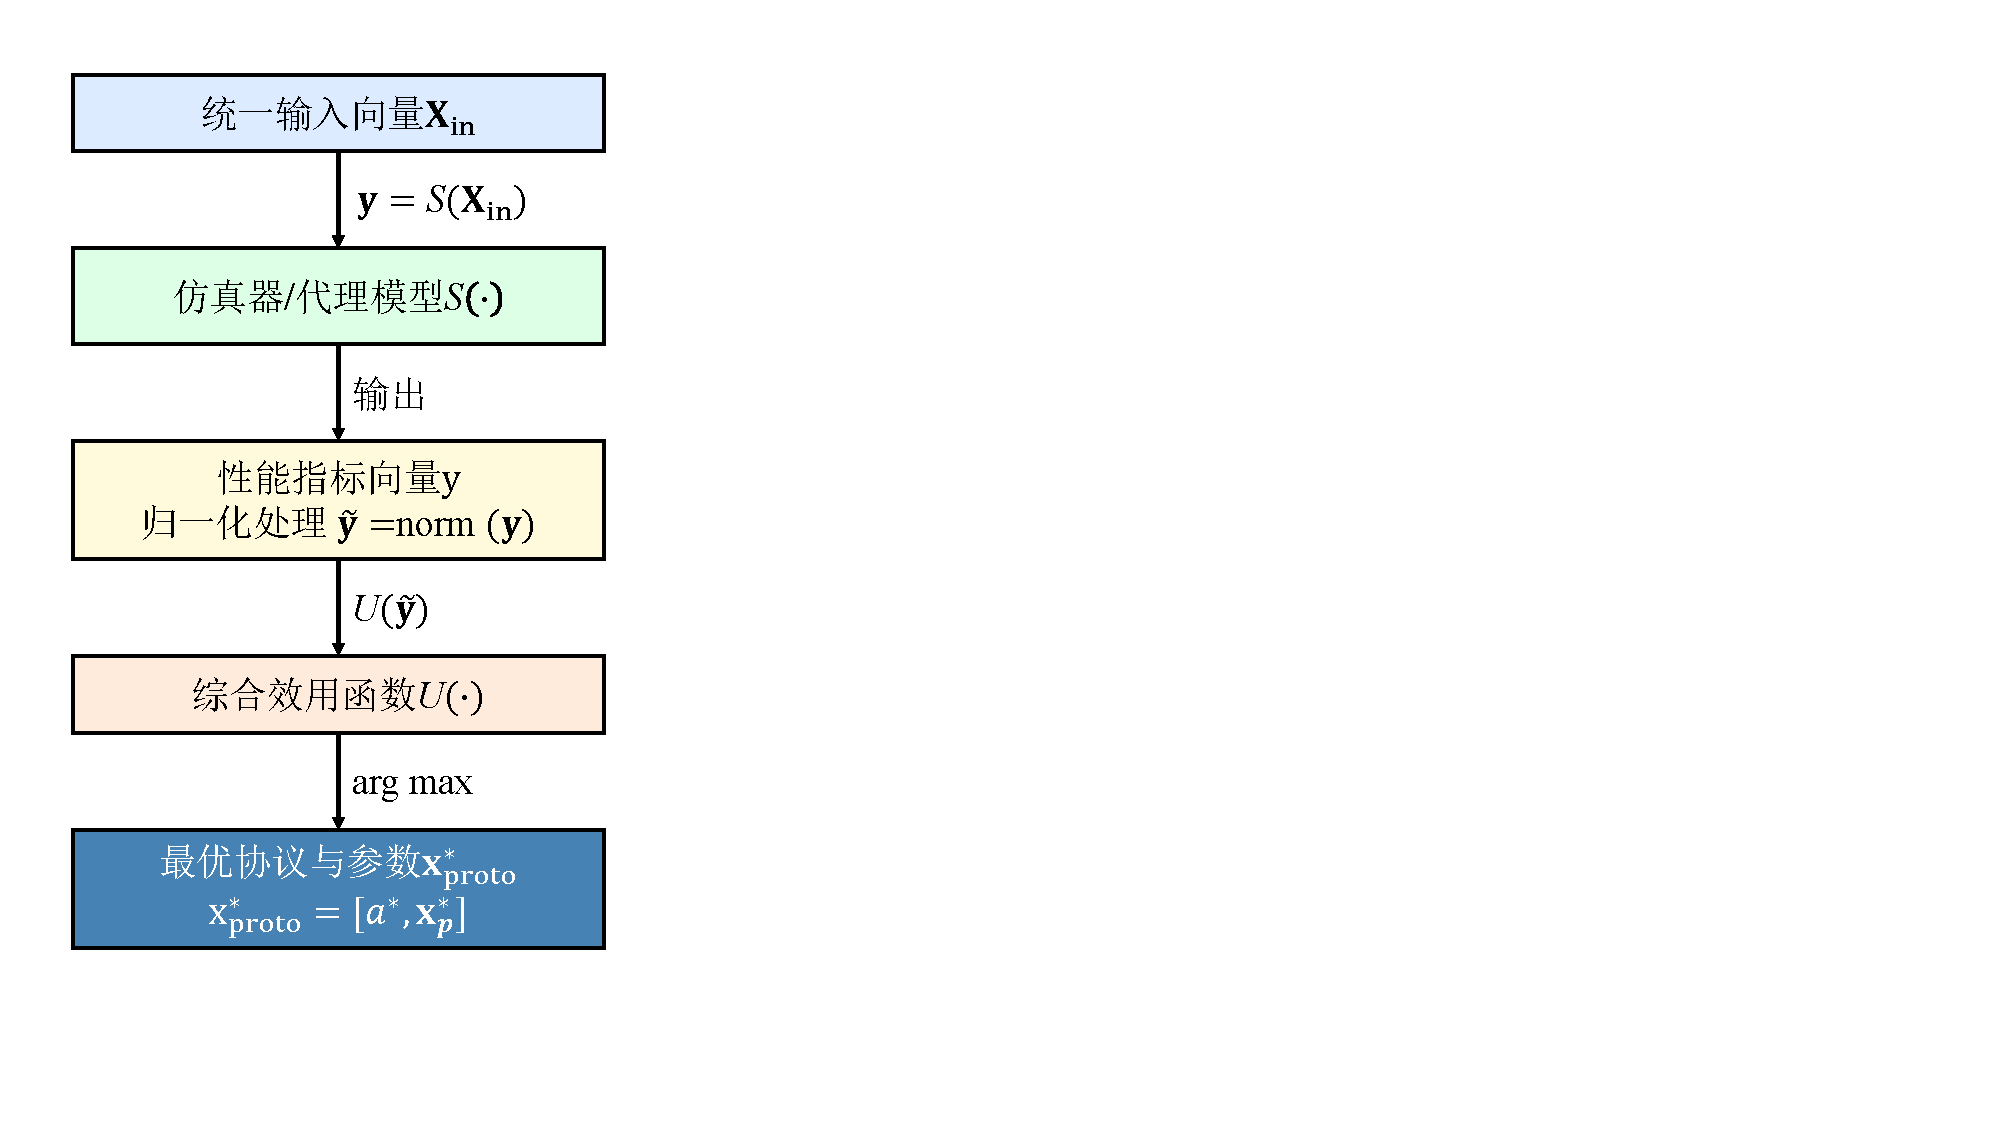
\includegraphics[width=0.3\textwidth]{figure/chap5/model1.pdf}
	\caption{不同协议在归一化网络平均到达率变化下的吞吐量对比}
	\label{fig:protocol_throughput_comparison}
\end{figure}

\textbf{吞吐量时延对比。} 
图~\ref{fig:protocol_throughput_comparison} 给出了不同协议随 $\hat{\lambda}$ 变化的输出吞吐量 $\lambda_{\mathrm{out}}$ 曲线。

\textbf{时延对比。} 
图~\ref{fig:protocol_delay_comparison} 展示了平均时延 $D$ 随 $\hat{\lambda}$ 的变化趋势。

\begin{figure}[htbp]
	\centering
	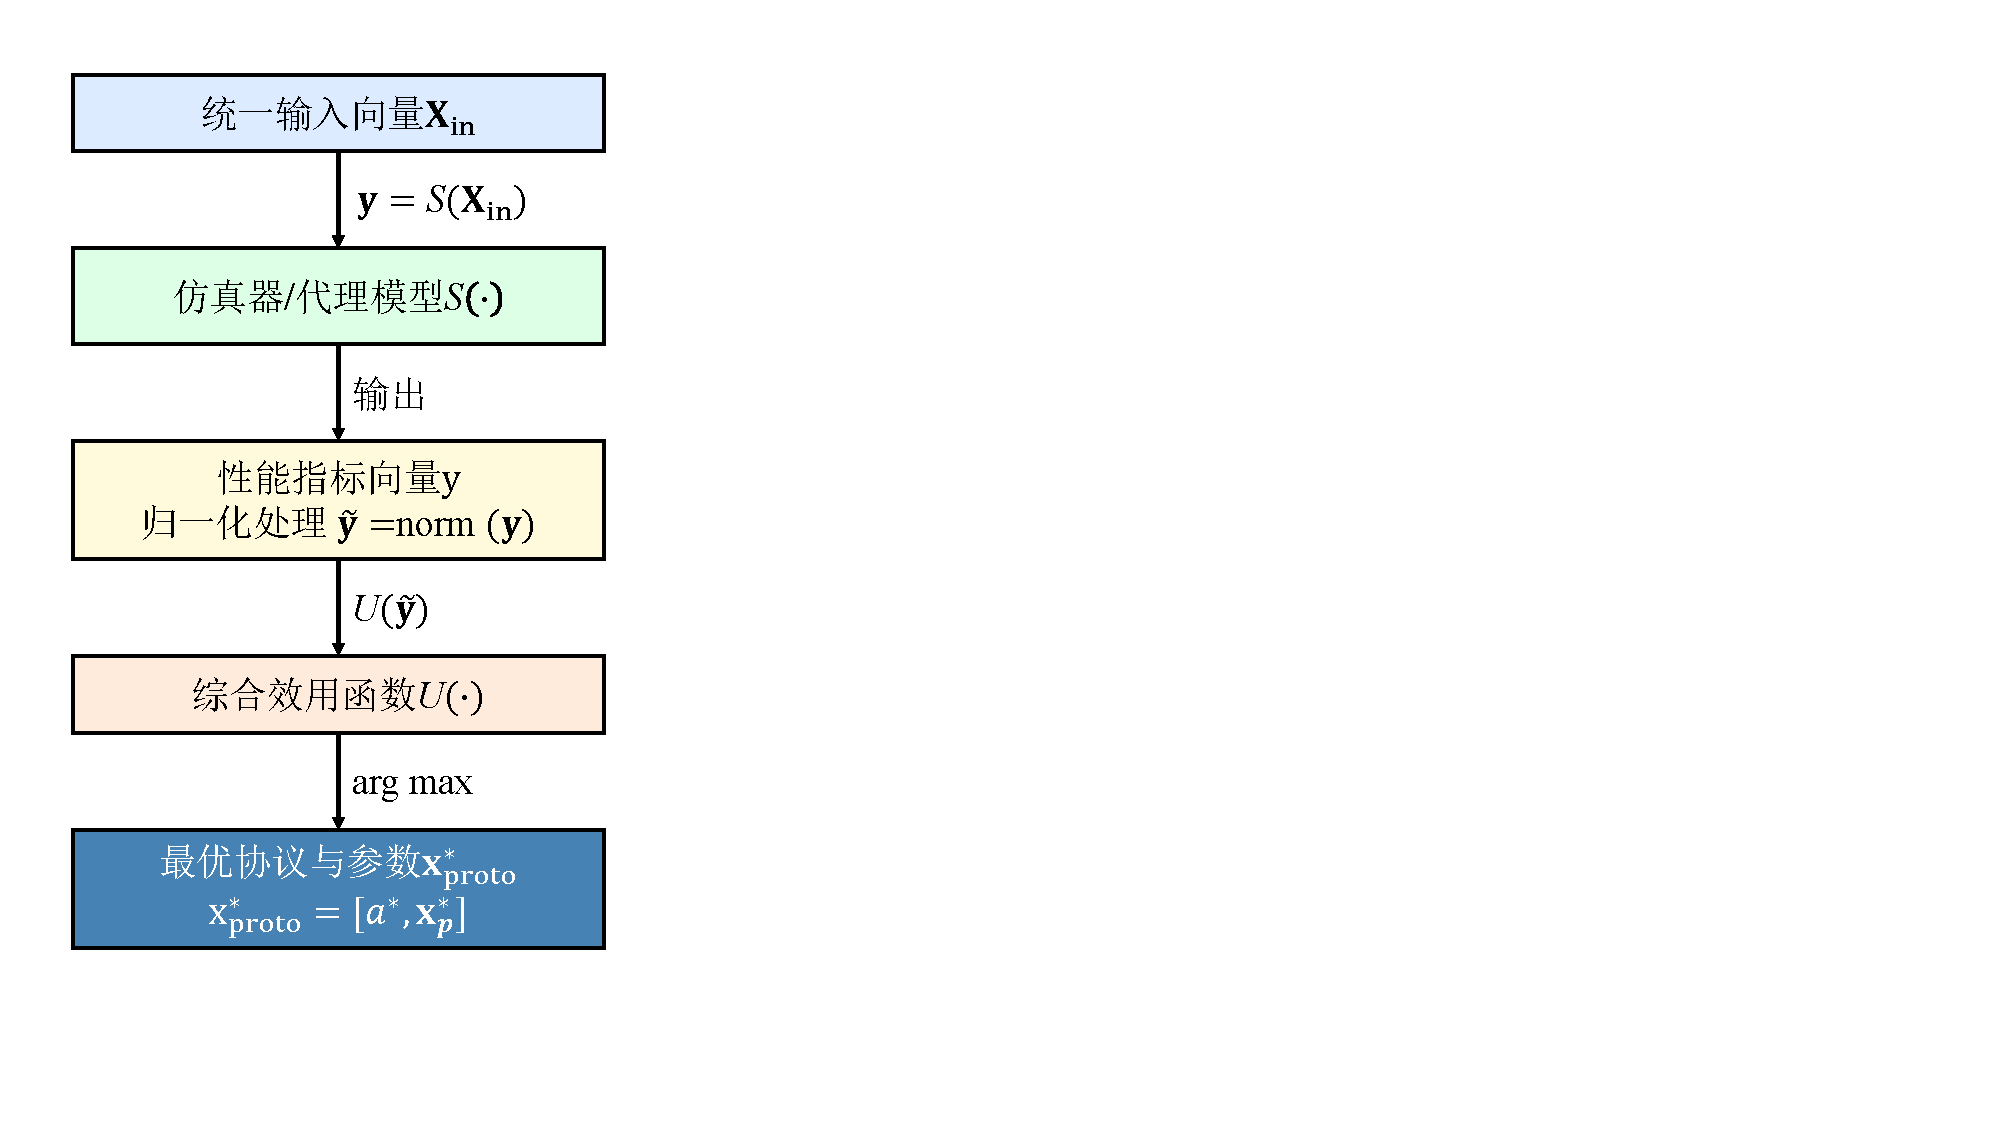
\includegraphics[width=0.3\textwidth]{figure/chap5/model1.pdf}
	\caption{不同协议在归一化网络平均到达率变化下的平均时延对比}
	\label{fig:protocol_delay_comparison}
\end{figure}




\textbf{公平性评估。} 
图~\ref{fig:protocol_fairness_comparison} 给出了公平性指标（Jain 指数）在不同协议下的变化特征。
\begin{figure}[htbp]
	\centering
	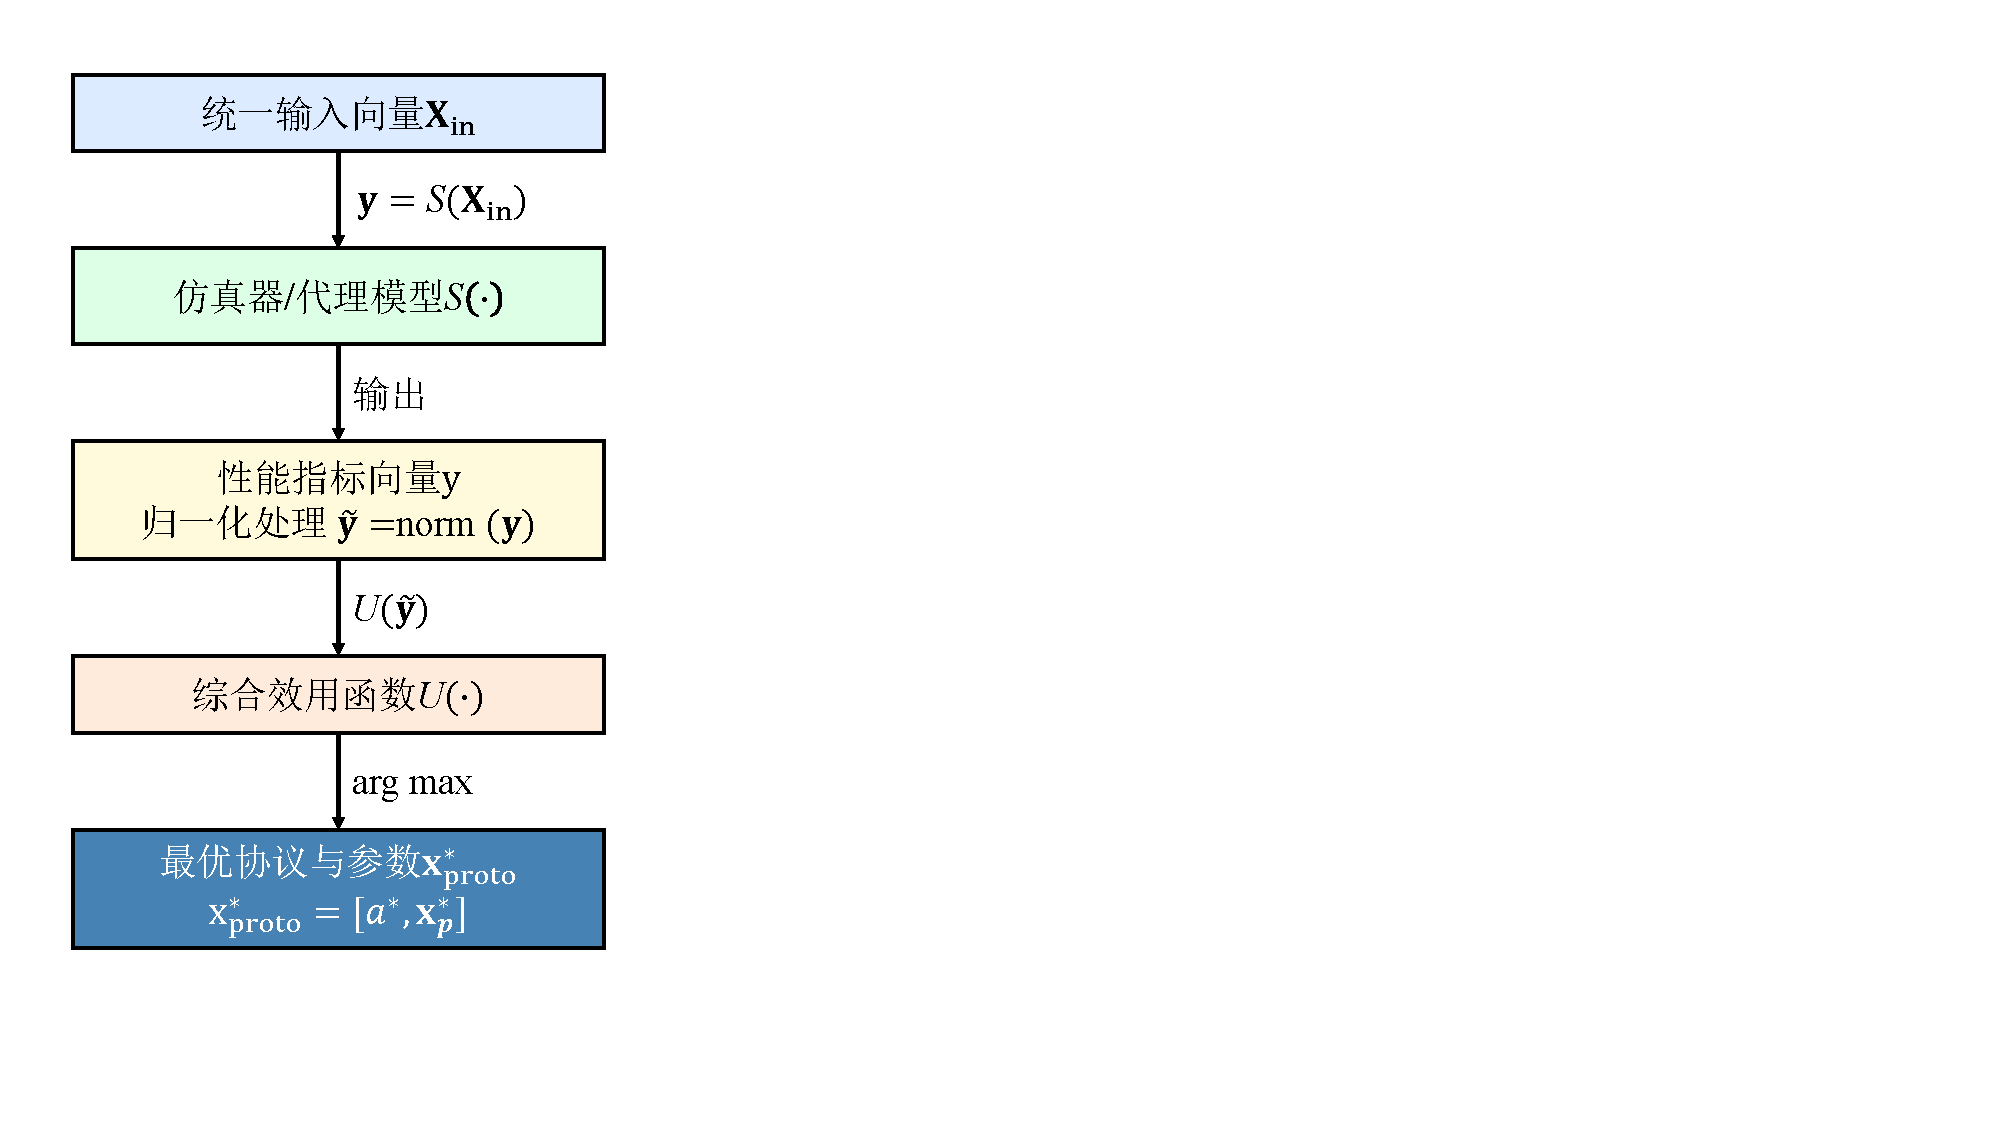
\includegraphics[width=0.3\textwidth]{figure/chap5/model1.pdf}
	\caption{不同协议的公平性指标对比（Jain 指数）}
	\label{fig:protocol_fairness_comparison}
\end{figure}

\textbf{综合效用评估。} 
为进一步量化多维性能的整体收益，图~\ref{fig:protocol_utility_comparison} 展示了基于式~\eqref{eq:chap5_constrained} 定义的综合效用 $U(\tilde{\mathbf{y}})$ 对比结果。

\begin{figure}[htbp]
	\centering
	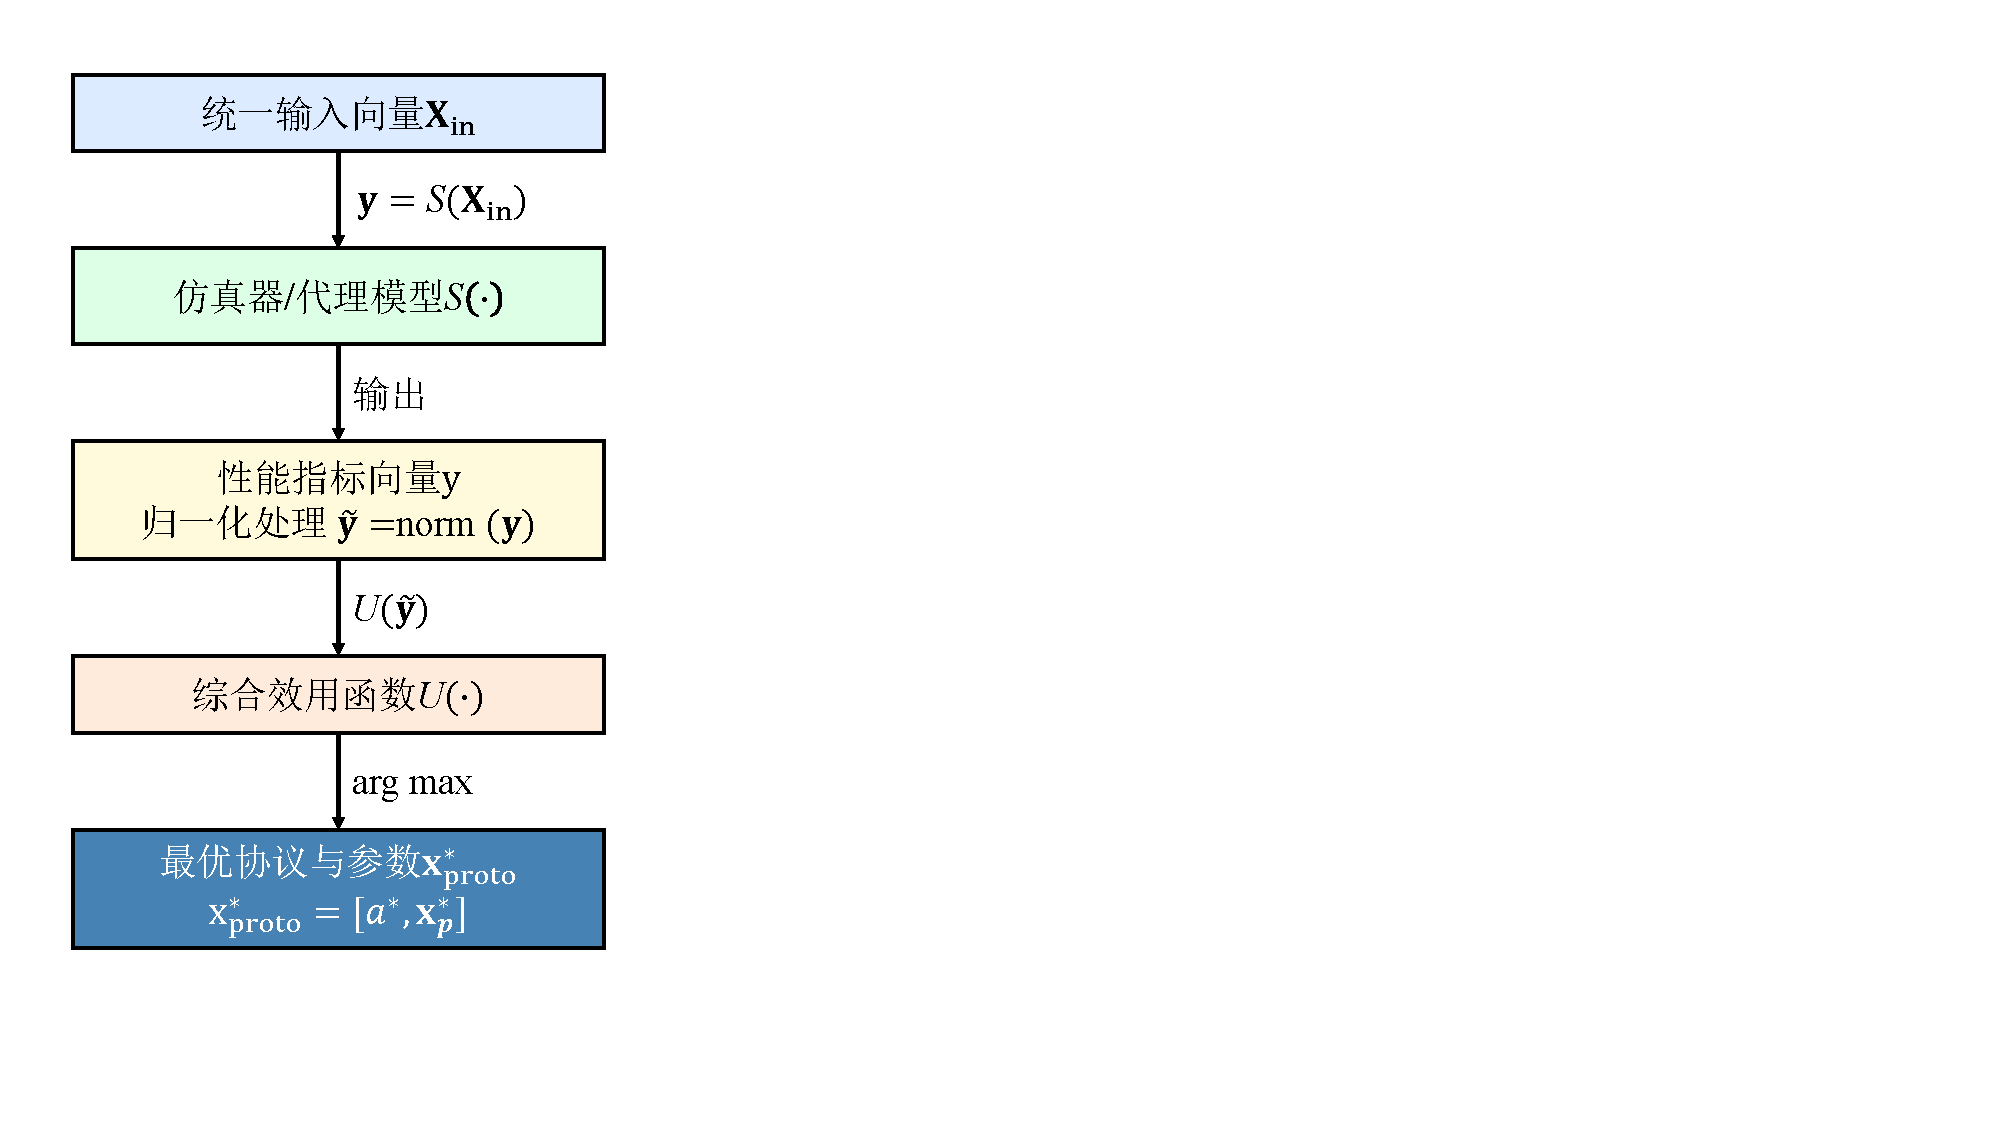
\includegraphics[width=0.3\textwidth]{figure/chap5/model1.pdf}
	\caption{不同协议的综合效用对比（权重：吞吐0.4，时延0.3，公平性0.2，资源0.05，实现0.05）}
	\label{fig:protocol_utility_comparison}
\end{figure}


% =========================================================
% 第 5.3 节：基于多任务深度学习的性能预测代理模型
% =========================================================

\section{基于多任务深度学习的性能预测代理模型}
\label{sec:mt_dnn_model}

虽然离散事件仿真器能够精确评估特定协议配置下的网络性能，但其时间成本高昂，单次仿真通常需要数秒至数分钟，严重制约了大规模参数空间的在线探索与实时优化。为解决这一瓶颈，本节基于5.2节构建的仿真数据集，设计并训练高效的深度学习代理模型。该模型采用多任务深度神经网络（MT-DNN）架构，能够利用单一网络同时预测吞吐量、时延、公平性等多维性能指标，实现从输入特征到性能评估的毫秒级快速映射，为后续的协议优化决策提供实时支持。

\subsection{基于硬参数共享的多任务网络架构}
\label{subsec:hard_sharing}

考虑到网络性能指标之间存在显著的物理耦合性，例如高负载状态通常同时对应吞吐量饱和与时延激增，独立的单任务模型往往忽略了这些内在关联，且训练效率低下。为此，本文设计了基于硬参数共享机制的神经网络架构，该架构在保持参数量可控的同时，能够有效学习多任务间的关联性。

\paragraph{架构设计原理}
硬参数共享架构由以下三个核心模块组成：

\begin{itemize}[leftmargin=*]
\item \textbf{输入归一化层}：采用 LayerNorm 对输入特征进行归一化，消除不同特征量纲差异，稳定梯度流。
\item \textbf{共享特征提取层}：包含2-3个堆叠的全连接层（可配置深度），每层配备 LayerNorm、GELU 激活函数与 Dropout。共享层学习所有任务通用的网络状态表征。
\item \textbf{任务特定头部}：每个任务配置独立的单层线性映射，实现从共享特征到任务输出的最终转换。
\end{itemize}

网络的数学表述如下。设输入特征维度为 $D_{\text{in}}$，共享层隐藏维度为 $D_{\text{hidden}}$（如128），共享层深度为 $L \in \{2, 3\}$。则共享特征提取过程为：
\begin{equation}
\mathbf{h}^{(0)} = \text{LayerNorm}(\mathbf{X}_{\text{in}} \odot \mathbf{m}),
\end{equation}
其中 $\mathbf{m}$ 为掩码向量，用于屏蔽无效参数分量。随后逐层计算：
\begin{equation}
\mathbf{h}^{(\ell)} = \text{Dropout}\left( \sigma\left( \text{LayerNorm}(\mathbf{W}^{(\ell)} \mathbf{h}^{(\ell-1)} + \mathbf{b}^{(\ell)}) \right) \right), \quad \ell = 1, \ldots, L,
\end{equation}
其中 $\sigma = \text{GELU}$ 为激活函数，Dropout 比率设为 0.1。第 $k$ 个任务的输出为：
\begin{equation}
\hat{y}_k = \text{Linear}(\mathbf{h}^{(L)}) = \mathbf{w}_k^{\top} \mathbf{h}^{(L)} + b_k,
\end{equation}
各任务无需额外激活函数，直接输出连续值。

表 \ref{tab:nn_architecture} 给出了具体的网络配置。

\begin{table}[htbp]
	\centering
	\caption{多任务代理模型的神经网络架构}
	\label{tab:nn_architecture}
	\renewcommand{\arraystretch}{1.25}
	\begin{tabular}{lll}
		\toprule
		\textbf{模块} & \textbf{结构配置} & \textbf{参数说明} \\
		\midrule
		\multirow{2}{*}{输入层} 
		& LayerNorm 
		& 特征归一化以稳定训练过程 \\
		& 掩码乘法 
		& $\mathbf{X}_{\mathrm{in}} \odot \mathbf{m}$，屏蔽无效或缺失特征 \\
		\midrule
		\multirow{5}{*}{共享隐藏层} 
		& FC + LayerNorm 
		& 维度映射 $D_{\mathrm{in}} \rightarrow D_{\mathrm{hidden}}$（如 128） \\
		& GELU + Dropout 
		& 非线性激活与正则化，Dropout 概率 $p=0.1$ \\
		& FC + LayerNorm 
		& 隐藏层维度保持 $D_{\mathrm{hidden}} \rightarrow D_{\mathrm{hidden}}$ \\
		& GELU + Dropout 
		& 激活与正则化 \\
		& 可选第 3 层
		& 深层模式下启用，用于提升模型表达能力 \\
		\midrule
		\multirow{2}{*}{任务输出头} 
		& 每任务独立全连接层 
		& 输出维度为 1 \\
		& 无激活函数 
		& 回归任务，直接输出连续值 \\
		\bottomrule
	\end{tabular}
\end{table}


参数量估计：在标准配置下（$D_{\text{in}} \approx 100$，$D_{\text{hidden}}=128$，$K=5$ 任务），模型参数量约 3000-4500，样本/参数比约 100-200，此比例可有效防止过拟合。

\subsubsection{前向传播过程}

输入特征 $\mathbf{X}_{\text{in}}$ 首先经过 LayerNorm 归一化，随后与掩码 $\mathbf{m}$ 进行元素级乘积，屏蔽当前协议不适用的参数维度。共享层按上述递推关系逐层提取抽象特征，每层输出通过 GELU 激活与 Dropout 进行非线性转换与正则化。最后，共享特征 $\mathbf{h}^{(L)}$ 分别输入各任务头，生成 $K$ 个任务的预测输出 $\{\hat{y}_1, \ldots, \hat{y}_K\}$，各任务输出均为标准化后的标量值。

\subsection{多目标优化与训练策略}
\label{subsec:training}

为了平衡多任务间的学习动态，模型训练采用多项策略\textbf{协同}实现：

\paragraph{加权多任务损失函数}
考虑到不同性能指标的数值尺度与学习难度差异，损失函数定义为：
\begin{equation}
	\mathcal{L}_{\text{total}} = \sum_{k=1}^{K} \omega_k \cdot \text{MSE}(\hat{y}_k, y_k^{\text{norm}}),
\end{equation}
其中 $y_k^{\text{norm}}$ 为标准化后的目标值（Z-Score 标准化），$\omega_k$ 为第 $k$ 个任务的权重系数。在实践中，关键性能指标（吞吐、时延、公平性）设权重为 1.0，而资源类指标（计算负荷、实现复杂度）设权重为 0.01，以强调性能优先。

\paragraph{数据增强与正则化}
在训练过程中，对输入特征添加高斯噪声进行数据增强，噪声标准差设为 0.03，模拟真实测量的随机波动。同时采用\textbf{强正则化}策略以防止过拟合：
\begin{itemize}[leftmargin=*]
\item Dropout 比率：0.1（每层共享特征提取）
\item L2 权重衰减：$5 \times 10^{-4}$（AdamW 优化器）
\item 梯度裁剪：梯度范数上界设为 1.0
\end{itemize}

\paragraph{优化与学习率调度}
采用 AdamW 优化器进行端到端训练，初始学习率设为 $1 \times 10^{-2}$。当验证损失连续 20 个 epoch 无改善时，采用 ReduceLROnPlateau 策略将学习率衰减为原来的 0.5 倍，最小学习率下界为 $10^{-6}$，避免学习过于缓慢。

\paragraph{早停机制}
监控验证集损失，当其连续 30 个 epoch 无改善时触发早停，保存验证损失最低时刻的模型检查点。此设计平衡了收敛速度与泛化性能。


\section{基于代理模型的快速预测与优化}

在代理模型 $f_{\phi}$ 训练完成后，原先耗时的协议优化问题便转化为一个可在毫秒级求解的数学优化问题。给定一个业务场景的流量特征 $\bm{x}_\text{traffic}$，目标是快速找到最优的统一参数向量 $\mathbf{x}_{\text{proto}}^*$（包含最优协议类型及其对应参数）：
\begin{equation}
	\mathbf{x}_{\text{proto}}^* = \arg\max_{\mathbf{x}_{\text{proto}}} U\big(f_{\phi}(\bm{x}_{\text{traffic}}, \mathbf{x}_{\text{proto}}, \dots)\big)
\end{equation}
由于代理模型 $f_{\phi}$ 的评估速度极快，我们可以采用高效的搜索算法来求解此优化问题。针对该问题的混合离散—连续参数空间特性，可以选择以下优化策略：
\begin{itemize}[leftmargin=*]
	\item \textbf{贝叶斯优化}：尤其适用于黑盒函数且评估成本较高的优化问题，在评估成本已显著降低的条件下，仍能有效平衡探索与利用，以较少迭代次数逼近全局最优解。
	\item \textbf{演化算法}：如遗传算法，能够并行地在参数空间中进行全局搜索，对目标函数的形态要求较低，鲁棒性较好。
\end{itemize}
通过这些先进的优化算法，系统能够在业务状态发生变化时，实现对接入策略的快速、自适应调整。

\section{本章小结}

本章提出了一种基于监督学习的智能协议与参数联合选择方法，旨在解决传统单一接入协议在复杂多变业务场景下的性能局限性。首先，我们设计了一个统一的接入框架，通过标准化的输入特征向量，对不同的业务流量、网络规模和协议参数进行统一建模。随后，为克服传统网络仿真的高时间成本，我们构建了代理模型，并利用多任务深度神经网络学习并复现从输入特征到多维性能指标的复杂映射关系。最后，基于训练好的、能够进行毫秒级预测的代理模型，将原先难以处理的协议优化问题转化为一个可由高效搜索算法求解的数学问题。

综上所述，本章通过统一框架设计、代理模型构建与快速优化求解，为实现随机接入机制的智能化和自适应化提供了完整的理论与实践基础。
